\documentclass[11pt]{article}
\usepackage[utf8]{inputenc}
\usepackage{tikz}
\usepackage{amsmath,amsfonts,amsthm}
\usepackage[vlined, ruled]{algorithm2e}
\usepackage{geometry}
\usepackage[noend]{algpseudocode}
\usetikzlibrary{bayesnet}
\usepackage[nottoc,numbib]{tocbibind}
\usepackage{enumitem,kantlipsum}
\usepackage{float}
\usepackage{titlesec}
\usepackage{natbib}
\usepackage{apalike}
\setcounter{secnumdepth}{4}

\titleformat{\paragraph}
{\normalfont\normalsize\bfseries}{\theparagraph}{1em}{}
\titlespacing*{\paragraph}
{0pt}{3.25ex plus 1ex minus .2ex}{1.5ex plus .2ex}

\setlength{\parskip}{1em}
\geometry{letterpaper,left=1.5in,right=1in,top=1in,bottom=1in}
\setlength\parindent{0pt}
\linespread{1.5}
\newcommand{\E}{\mathrm{E}}
\newcommand{\Var}{\mathrm{Var}}
\newcommand{\N}{\mathcal{N}}
\newcommand{\tr}{tr}

\begin{document}
\pagenumbering{gobble}
{\centering
  \textbf{The High-Order Brain Dynamics (HOBD) Model}\par
  A Thesis\par
  Submitted to the Faculty\par
  in partial fulfillment of the requirements for the\par
  degree of\par
  Master of Science\par
  in\par
  Computer Science\par
  by\par
  Hao Chang\par
  DARTMOUTH COLLEGE\par
  Hanover, New Hampshire\par
  May, 2017\par
}
\vspace{5mm}
\setlength{\parskip}{0em}
\begin{flushright}
Examining Committee:\par
\vspace{5mm}
$\rule{5cm}{0.15mm}$\par
Hany Farid\par
\vspace{5mm}
$\rule{5cm}{0.15mm}$\par
Qiang Liu\par
\vspace{5mm}
$\rule{5cm}{0.25mm}$\par
Jeremy Manning\par
\end{flushright}
\setlength{\parskip}{1em}
\newpage


\null\par
\newpage
\pagenumbering{roman}
\section{Abstract}
Recent researches focused on analysis of the dynamic correlation structures of brain activities has achieved monumental breakthroughs in improving our understanding of the human brain. Thus, we hypothesize exploration of high order functional connectivities within the brain---the correlation within correlation structures---could potentially reveal more information on the dynamics behind brain functions. To achieve this, we present the High-Order Brain Dynamics (HOBD) model, which incorporates informations from multiple orders of brain functional connectivity to gain a more comprehensive understanding of how the brain responds to controlled stimuli. The HOBD model also introduces two new methods: TimeCorr, which revolutionizes the way functional connectivity is calculated, and TimeCorr Level Up, a new scalable solution to retrieving functional connectivity at high orders. Through the lens of the the HOBD model, we discovered important patterns in how stimulus-driven brain dynamics information is represented by each level of functional connectivity, as well as how information of different orders of functional connectivity can potentially complement each other to increase the amount of information we can decode from the brain.

\newpage
\section{Acknowledgements}
Firstly, I would like to thank my mentors Professor Jeremy Manning of the Psychological and Brain Sciences Department at Dartmouth College and Professor Qiang Liu of the Computer Science Department at Dartmouth College. Professor Manning and Professor Liu were great inspirations for me throughout this project. Their deep understanding of their respective fields and constant flow of bright ideas really expanded my understanding of what it means to love and excel at what I want to do. Professor Manning and Professor Liu provided timely guidance whenever I was in need and constantly encouraged me to try out new ideas and to reach for higher standards.

Secondly, I would also like to thank Professor Hany Farid of the Computer Science Department at Dartmouth College. Professor Farid kindled my first spark of interest in computer science and pushed me to pursue graduate eduction at Dartmouth. He has been a role model for me throughout my education at Dartmouth and will always be an inspiration for me in my future pursuits in life.

Thirdly, I would like to thank Andy Heusser and Kirsten Ziman in the Contextual Dynamics Laboratory in the Neuroscience Department at Dartmouth College. Andy and Kirsten played crucial roles in helping me overcome my lack of experience in neuroscience related researches. Their patient and timely assistance helped me through many difficulties at crucial stages of my research.

Fourthly, I would also like to acknowledge Dilin Wang, Jun Han and Yihao Feng in the DartML lab of the Computer Science Department at Dartmouth College. Their door were always open whenever I ran into a trouble spot or had a question about my research or writing.

Finally, I must express my very profound gratitude to my parents for providing me with unfailing support and continuous encouragement throughout my years of study and through the process of researching and writing this thesis. This accomplishment would not have been possible without them. Thank you.

\newpage
\tableofcontents
\newpage
\pagenumbering{arabic}

\section{Introduction}
Human beings have an insatiable desire to understand, not only the things around us, but also ourselves. Why do we behave and respond the way we do \citep{hasson2012}? How do we learn and adapt \citep{hasson2004}\citep{hasson2005}? What do we believe or value \citep{Greene01}? How does social context affect the way we think \citep{Matthew2015}? These questions have mesmerized wise men for thousands of years, and the answers continue to evade us. For many of us, the key to understanding human behavior lies in our brain, the central hub of all our thoughts and decision making. So, when a new technology emerged allowing us to study the brain in a quantitative manner, it opened countless doors of opportunities for those who possessed an aptitude for quantitative analysis and a hunger to learn more about our own identity.

Functional Magnetic Resonance Imaging, often referred to as fMRI, was first discovered and applied as a brain mapping method in 1990 by Seiji Ogawa \citep{Ogawa90}. Since then, this technology quickly popularized among Brain Science related research due to its unprecedented low health risk to subjects and its ability to accurately translate brain activities into highly-structured quantitative data \citep{Logothetis01}. Once the highly abstract brain activities are converted into signs and digits, exploring patterns in the brain simply devolves into highly intricate mathematical problems. For example, by treating each brain fMRI image as a feature vector, Machine Learning algorithms trained on a subset of the data can learn to identify cognitive patterns (e.g. which part of a movie someone is watching), and be used to extract similar patterns from held-out brain images \citep{Norman06}\citep{peterson12}\citep{peterson17}. These applications typically treat each brain image in isolation, and attempt to decode patterns of activities associated with each of several candidate brain states. However, important stimulus-driven activities in fMRI data are often obscured by noises created by non stimulus-driven neural activity \citep{peterson11}, thus limiting the effectiveness of any decoding effort. To address this issue, new branches of research have been emerging that specifically focus on the extraction of useful information from noisy brain fMRI data by treating brain fMRI images as time series of dynamic activities, and one of the most fruitful directions involves analyzing functional connectivities within the brain \citep{peterson19} \citep{peterson20}.

The brain can be divided in various ways---according different rules of systemization (by functionality, organization, activity patterns, etc)---into a set of regions, and functional connectivity describes the correlation between the time series of activations each pair of brain regions exhibits. When we observe the brain, the neural activities can appear incredibly complex. But the mechanics of brain are far from random, rather, the dynamic patterns of the activities our brains exhibit are highly structured. Presumably, this mirrors the complex but highly structured nature of our internal thoughts and experiences. Many past studies on functional connectivity have focused on using resting state data (images taken as participants rest in the scanner with their eyes open) to estimate a single correlation matrix for each person \citep{peterson9}. Each subject's correlation matrix provide a rich database for mapping the relations among brain processes and their contributions to perception, action and cognition \citep{Bassett2017}. These cognitive information were then used as identifiers to relate and compare patterns in subjects' brain activities to patterns in subjects' behaviors on various tasks \citep{Turke13}\citep{Rubinov2010}\citep{peterson10}.

Recent research efforts have revealed that important cognitive information is contained in the temporal correlational structure of time series brain activities \citep{davidson2016}, and as a result, approaches focusing on understanding the brain through analysis of dynamic brain functional connectivities begun to rapidly emerge \citep{Nigam2016}\citep{Hutchinson2013}. One of the most significant advancements comes from a recent paper by Uri Hasson's group, which casts functional connectivity as a dynamic process that changes from moment to moment depending on the specific experience of that moment \citep{hasson2016}. When analyzing the brain functional connectivity of one experimental subject in isolation, one can examine how (or whether) the correlational structure of these activity patterns (across a given set of brain regions) varies according to the cognitive task the subject is performing. The paper also presents the revolutionary idea of inter-subject functional correlation (ISFC) analyses, which analyzes the functionally connectivities across multiple subjects to isolate stimulus-dependent inter-regional correlations from random neural activities and non-neuronal noise. Dynamic functional connectivity and ISFC analysis were successfully applied by the Contextual Dynamics Lab in their most recent paper on hierarchical topographic factor analysis (HTFA) in brain decoding tasks. The HTFA also discovered that high-order functional connectivity patterns and basic brain activation patterns contain partially non-overlapping information about stimulus-driven brain dynamics, which was the main inspiration for the investigations behind this thesis \citep{jeremy2017}.

Although functional connectivity analyses of brain data has evolved significantly \citep{olaf2005}\citep{khambhati2017}, there are still three fundamental limitations to past approaches:

Firstly, \textbf{correlation matrices are not scalable.} Examining pairwise correlation in brain data containing $n$ regions (henceforth interchangeable with ``voxels") produces a correlation matrix with $n^2$ entries. When n is large (e.g. the number of brain regions in an fMRI volume), the full correlation matrix can become unwieldy to compute with \citep{Rubinov2010}\citep{Betzel2017}\citep{Craddock2012}\citep{Yeo2011}. Furthermore, if one wishes to examine higher-order patterns (e.g. how correlations between correlations change over time), the storage requirements of the resulting patterns increase exponentially.

Secondly, \textbf{the sliding window approach is not well suited to the study of dynamic activity.} Most approaches to calculating functional connectivity uses the sliding window method, where the correlation function is applied on the brain activations of time points within a window of set length to calculate the functional connectivity at the central time point. To calculate functional connectivity of following time points, the window is shift forward one time point at a time until the edge of the window reaches the end of the time series \citep{enrico2011}\citep{elena2012}. One disadvantage of the sliding window approach is that, for a time series of length $t$ and a window length of $l$, it can only retrieve the functional connectivity of $n=t-l$ time point, thereby losing information on $l$ time points. Although many practical applications use buffers to make up for the loss, repeated application of the sliding window approach on the same dataset—--e.g. calculating the correlation of the correlation between nodes—--is impractical. In addition, the sliding window approach provides only a poor approximation of the moment-by-moment patterns at the heart of these representations.

Lastly, \textbf{important information may exist beyond voxel activations and their first level functional connectivity.} The brain is a network of seemingly autonomous nodes that are actually intricately interconnected. Useful information about the brain may exist within interactions between interactions between brain regions (2nd order functional connectivity), interactions between interactions between interactions (3rd order functional connectivity), or in even higher orders of functional connectivity. To fully grasp the functions of a single brain region in the network, it is crucial to understand of its activities relative to the richly woven network that supports it. Therefore, incorporating information from higher order dynamics could potentially improve the quality of brain analysis.

Here, we present the High-Order Brain Dynamics (HOBD) model, a new perspective that seeks to achieve a deeper understanding of the brain through analysis of the dynamics behind higher order brain interactions and how these different ``levels" of interaction between brain structures is represented in the brain. To efficiently access and analyze brain dynamics at higher levels, the HOBD model revolutionizes functional connectivity calculation methods and creates a means to repeatedly ``level up" brain dynamics information, computing higher level functional connectivity from low level information. These changes have notably improved the recovery accuracy of brain correlation structures, and significantly increased the decoding capabilities of existing brain datasets.

Firstly, to find an effective replacement for the widely used sliding window method, we designed TimeCorr, an intuitive method that finds its inspiration directly from the fundamental correlation function. Like the sliding window method, TimeCorr is able is able to recover functional connectivity from fMRI brain images with similar if not higher accuracy. But TimeCorr goes beyond the sliding window method by (a) not requiring buffers for its calculations, thereby avoiding data loss, (b) offering extra stability by using all the time points in the time series for calculations at every time point, (c) providing the option to adjust the locality and fluidity of results through changing the resolution parameter.

To achieve the functionalities mentioned above, TimeCorr makes use of the Gaussian distribution. By attaching a Gaussian coefficient to components at each time point in the series, TimeCorr is able to allocate the amount of influence each neighboring time point has on the calculation of the correlations at the Guassian center. As the Gaussian center (highest density/coefficient) is always at the time point of interest, TimeCorr guarantees to return highly accurate approximations of the temporal ground truth. In addition, the user can choose to have more fluidity in the results by choosing coefficients from a Gaussian distribution with a larger variance; or higher resolution and more locality by choosing coefficients from a distribution with a smaller variance.

Secondly, we designed a ``level up" method that applies TimeCorr, Inter-Subject Functional Connectivity (ISFC) and Principle Component Analysis (PCA) to calculate higher order functional connectivity. To overcome the problem of scaling and to enforce uniformity for inter-levels analysis, we use TimeCorr on each subject to calculate functional connectivity from previous level activations and then reduce the results to an arbitrary number of voxels to represent the activations for the next level. As TimeCorr avoids data loss in calculating functional connectivity and PCA maintains an uniform number of activations after each ``level up", we are able to obtain functional connectivities up to the $10^{th}$ order while ensuring linear scaling in storage and computation.

We believe that different orders of functional connectivity represents information on different aspects of brain dynamics, and incorporating knowledge of the higher-order structures of the brain will expand present brain decoding capabilities. To measure the amount of information present at each level, we introduce decoding accuracy, a testing parameter that describes the proportion of time points in a subject's functional connectivity that have highest correlation with the same time point in the ISFC of all other subjects. We are interested in how decoding accuracy changes as we reach higher order functional connectivity. Although we presumed brain dynamics of different subjects would converge as we get to higher orders, resulting in increasing decoding accuracy, reality proved otherwise. This is shown and discussed in more detail in the Decoding Analysis section of our results.

To carry out an in-depth evaluation of the effectiveness of the HOBD model, we also conducted the Multi-Level Mixture Analysis. This study aims to understand how the dynamic information of different levels of interactions between brain regions can be used in unison (weighted sum) to improve decoding capabilities of existing brain fMRI datasets. In the Multi-Level Mixture Analysis section of our results, we provide a side by side comparison that highlights the improvements achieved by our mixture model. In the process of finding the mixture model that maximizes decoding accuracy, we also explored the utility of each level of brain dynamics through analysis of the distribution of optimal weights for each level. The methods and findings will be discussed extensively in the results section.

\newpage
\section{Model Description}
The High-Order Brain Dynamics model seeks a new perspective to understanding the dynamics behind stimulus-driven brain activities. Utilizing the capabilities and advantages of TimeCorr and ``Level Up", the HOBD model attempts to incorporate information on high-order brain dynamics into its analysis of brain dynamics.

\subsection{Single Subject TimeCorr}
The TimeCorr method was designed for the purpose of replacing the sliding window method as a lossless alternative to achieve more accurate calculation of functional connectivity (the correlation structure between brain regions within a subject's brain) from brain fMRI data. The sliding window method operates by applying the correlation calculation function on a block of data centering on the time point of interest $t$ and spanning $L_w$ time points, where $L_w$ is the sliding window length and must be of considerable magnitude for the sliding window method to achieve respectable accuracy. However, due to its inherent design flaw, using the sliding window method on a dataset of time length $T$ could only yield functional connectivity for $T-L_w$ data points, a loss not insignificant due to the typical magnitude of $L_w$. Thus, as calculating high order functional connectivity involves repeated application of the method of correlation calculation on the dataset, using the sliding window method would result in rapid deterioration in the amount of usable data. In addition, as the sliding window method uses a long block of data for correlation calculation, it can only achieve a rough approximation of the general average in the block and not the instantaneous truth at each time point.

To solve these problems, we designed the TimeCorr method, which finds inspiration from the fundamental correlation function. Instead of isolating only a block of time points, TimeCorr effectively utilizes information from the entire dataset for functional connectivity calculation at every time point. To ensure locality of TimeCorr's results, every term is multiplied by a weight drawn from a normalized Gaussian density function so that each time point influences the calculation of functional connectivity at the time point of interest $t$ proportionally to its distance from $t$. This adaptation of the correlation function effectively eliminates results repetition at the beginning and end of the time series, thereby increasing the number of output time points to equal to the number of inputs and avoiding any data loss. In addition, through the application of Gaussian density coefficients, TimeCorr gives more significance to information closer to the time point of interest in its calculations, thereby ensuring a more accurate estimation of instantaneous correlation.

\large{\textbf{Formal Definition}}

\normalsize
Given a single subject's brain activation matrix with T time points and V voxels, to apply TimeCorr:

\begin{enumerate}
\item Base on the amount of influence neighboring time points should have on the calculation of the functional connectivity at each time point, choose variance $\sigma$ for the Gaussian density function to generate coefficients.

\item For each time point t:
\begin{enumerate}
\item Using a Gaussian density function of variance $\sigma$ and mean $t$, generate an array of coefficients $w_t$ of length T.

\item For each voxel, element-wise multiply its activation time sequence $a_i$ by the coefficients array to create a weighted activations array $S^i_t$.

\item Find the temporal correlation between voxel i and voxel j at time point t through the equation:

\begin{align*}
C(S^i_t,S^j_t) = \frac{1}{Z}\frac{\sum_{l=0}^T (S_l^i - \bar{S^i_t})\cdot(S^j_l - \bar{S^j_t})\cdot \mathcal{N}(l|t,\sigma)}{\sigma_{S_t^i} \cdot \sigma_{S_t^j}}
\end{align*}
Where
\begin{align*}
Z &= \sum_{l=0}^T \mathcal{N}(l|t,\sigma)\\
\bar{S^i_t} &=\frac{1}{Z} \sum_{l=0}^T S^i_l \cdot \mathcal{N}(l|t,\sigma)\\
\sigma_{S_t^i} &=\sqrt{ \frac{1}{Z}\sum_{l=0}^T (S_l^i-\bar{S_t^i})^2 \cdot \mathcal{N}(l|t,\sigma)}\\
\end{align*}
\item Repeat above process for every voxel pair to create correlation matrix for time point t
\item Convert the correlation matrix at every time point to its inverse squareform format, outputting an array of size $T$ by $(V^2-V)/2$ dimensional matrix, where $T$ and $V$ represent the time length and voxel count of the dataset.
\end{enumerate}
\end{enumerate}

The Gaussian variance parameter V gives the user the extra freedom to customize the desired level of resolution for correlation calculation. If a large variance is chosen, the influence of neighboring time points on the calculation of functional connectivity at each time point is increased, thereby adding smoothness and stability to the resulting functional connectivity time sequence and providing a more accurate representation of the general trend. But if a small variance is chosen, most of the weight will be placed on the time point of interest and its immediate neighbors, and so the resulting functional connectivity time sequence will have more emphasis on local accuracy. After experimenting with different setups, we discovered that choosing a Gaussian variance equal to the minimum between 1000 and the total number of time points achieves a good balance between locality and fluidity. This finding will be discussed in more detail in the Results section.

In contrast to the sliding window method, which is widely considered to be the golden standard for fMRI functional connectivity calculation, the TimeCorr approach is able to more accurately retrieve the temporal correlation at each time point without loss of important data. This advantage makes it possible to ``level up" to higher order functional connectivities---progressively finding the correlation of correlations---and explore dynamics and patterns heretofore untouched. We will go into more detail about the ``level up" process and high order functional connectivity in the ``Multi-Subject TimeCorr Level Up" section.

\subsection{TimeCorr Inter-Subject Functional Connectivity}

Inter-Subject Functional Connectivity (ISFC) is the functional connectivity between brain regions of different subjects \citep{jeremy2017}\citep{hasson2016}. The patterns recovered by ISFC is analogous to single subject functional connectivity (which reflect the correlational structure across brain regions within an individual's
brain), but they should reflect only activities that are specifically stimulus-driven. For every subject, we compare its brain activations time sequence $a_i$ with the average activations of all other subjects $a_{-i}$. Through the process of averaging the activations of multiple subject, we dampen random noises and emphasize activities that are common across all subjects, which are usually stimulus-dependent. Therefore, when we calculate the functional connectivity matrix between subject activation $a_i$ and the average response from the rest of the participants $a_{-i}$, the functional connectivity we calculate are more likely to reflect activities that are stimulus-driven.

Furthermore, after we obtain the functional connectivity matrix between each subject and the average of their counterparts, we use Fisher Z-transformation to average the results from all the subjects. In addition to the noise-dampening and stimulus-enhancing effects that comes with averaging, we are also able to gain an unbiased view of the overall stimulus-driven functional connectivity patterns across all subjects within our analysis. Fisher Z-transformation is applied in the averaging process as a means to stabilize and reduce approximation variance and return a less biased result than that of directly averaging correlations.

\large{\textbf{Formal Definition}}

\normalsize
Given an activations dataset containing $N$ subjects, each with T time points and V voxels, to apply TimeCorr ISFC:
\begin{enumerate}
\item Determine the desired temporal resolution for calculation and select $\sigma$, the variance of the Gaussian density function for TimeCorr coefficients generation.
\item For each subject s,
\begin{enumerate}
\item Find the average activation of all other subjects:
\begin{align*}
O_s=\frac{\sum_{i\neq s}^N S_i}{N-1}
\end{align*}
where $S_i$ represents the activation matrix for subject $i$ and $N$ represents the total number of subjects.
\item Find the functional connectivity between the brain activations $S$ for subject $s$ and the average activations of all other subjects $O$ using TimeCorr ISFC with variance $\sigma$. The correlation between $S^i_t$---activation of voxel i for subject $s$ at time $t$---and $O^j_t$---average activation of voxel $j$ of all other subjects at time points $t$---is obtained through the following equation:
\begin{align*}
C(S^i_t,O^j_t) = \frac{1}{Z}\frac{\sum_{l=0}^T (S_l^i - \bar{S^i_t})\cdot(O^j_l - \bar{O^j_t})\cdot \mathcal{N}(l|t,\sigma)}{\sigma_{S_t^i} \cdot \sigma_{O_t^j}}
\end{align*}
Where
\begin{align*}
Z &= \sum_{l=0}^T \mathcal{N}(l|t,\sigma)\\
\bar{S^i_t} &=\frac{1}{Z} \sum_{l=0}^T S^i_l \cdot \mathcal{N}(l|t,\sigma)\\
\bar{O^i_t} &=\frac{1}{Z} \sum_{l=0}^T O^i_l \cdot \mathcal{N}(l|t,\sigma)\\
\sigma_{S_t^i} &=\sqrt{ \frac{1}{Z}\sum_{l=0}^T (S_l^i-\bar{S_t^i})^2 \cdot \mathcal{N}(l|t,\sigma)}\\
\sigma_{O_t^i} &=\sqrt{ \frac{1}{Z}\sum_{l=0}^T (O_l^i-\bar{O_t^i})^2 \cdot \mathcal{N}(l|t,\sigma)}\\
\end{align*}
\item Repeat the above process for every pair of voxels, for every time point to obtain a time series of correlation matrices
\end{enumerate}
\item Element-wise apply Fisher Z-transformation to the correlation matrices for each subject at each time points to obtain the corresponding Z-correlation matrices:
\begin{align*}
z = \frac{1}{2}\ln(\frac{1+r}{1-r})
\end{align*}
\item Element-wise average the Z-correlation matrices $Z_i$ across all subjects:
\begin{align*}
S_Z = \frac{1}{N}\sum^N_{i=1}Z_i
\end{align*}
\item Element-wise apply inverse Z-transformation to the average Z-correlation matrix to obtain the TimeCorr ISFC matrix:
\begin{align*}
\text{TimeCorr ISFC} = \frac{\exp(S_Z+S_Z^T)-1}{\exp(S_Z+S_Z^T)+1}
\end{align*}
\item Convert the correlation matrix at every time point to its inverse squareform format, and output a $T$ by $(V^2-V)/2$ dimensional matrix containing the average functional connectivity of all subjects in the dataset, where $T$ and $V$ represent the time length and voxel count of the dataset, respectively.
\end{enumerate}

\subsection{Multi-Subject TimeCorr Level Up}
The multi-subject TimeCorr Level Up process utilizes the functionalities of the single-subject TimeCorr method to extract high-order brain dynamics patterns from brain fMRI data. Due to the data-loss flaw of the sliding window method, research related to functional connectivity heretofore have been largely limited to analysis of raw fMRI activations and first order functional connectivity. However, with the availability of TimeCorr, we are able to repeatedly find higher order functional connectivity of an fMRI dataset without fear of losing data with each ``level up". This advantage allows us to explore higher order dynamic patterns within the brain that was previously impossible to access.

The concept of ``leveling up" involves repeatedly finding the correlation of correlations of brain activity. Given a brain fRMI dataset, we designate the raw activations as level 0 and the functional connectivity (correlation structure) of the raw activations as level 1, the result of ``leveling up" from level 0 (henceforth ``level" and``order" are interchangeable). Hereafter, given a matrix containing the functional connectivity of the $n^{th}$ order, we can use the TimeCorr Level Up method to find its correlation structure and obtain the $n+1^{th}$ order functional connectivity.

In addition to effectively retaining all relevant data, the Multi-Subject TimeCorr Level Up method also presents a scalable solution to large datasets. Normally, for an input dataset of $V$ voxels (brain regions), the first order functional connectivity would occupy $V^2$ space and every additional level of functional connectivity would involve an exponential increase in storage requirement. In order to circumvent this problem, the Multi-Subject TimeCorr Level Up method first finds the inverse square-form (vectorized array containing half of the non-diagonal elements of a square matrix) of the correlation matrices for every time point in the ``level up" output, and then uses PCA to further reduce the result to a matrix of $T$ by $V$ dimensions, where $T$ and $V$ represent the time length and voxel count of the input dataset. This solution ensures all orders of functional connectivity derived from the same dataset will have the same dimensions. In addition, the application of PCA further guarantees that only the most principle components of each functional connectivity matrix is retained for further analysis.

\large{\textbf{Formal Definition}}

\normalsize
Given a brain activation matrix or a $n^{th}$ order functional connectivity matrix containing N subjects, V voxels and T time points, the Level Up function

\begin{enumerate}
\item Apply single-subject TimeCorr on the activation matrix of each subject to obtain their corresponding functional connectivity matrices

\item Concatenate the correlations matrix for each subject from the previous step together along the first (time) dimension into a single matrix of dimensions $(N*T)$ by $V$

\item Apply PCA on the concatenated matrix from the previous step to obtain a reduced representation of the correlation matrix

\item Separate the reduced correlation matrix from the previous step into data for each subject to obtain a 3-D matrix of size $N$ by $T$ by $V$, where $N$, $T$ and $V$ represent subject count, dataset time length and voxel count, respectively

\item Repeat the above process on the output to level up again

\end{enumerate}

By concatenating the functional connectivity of all subjects into a single matrix before PCA reduction, we guarantee consistency in the orientation of principal components in the reduced functional connectivity matrix across all subjects. As a result, although the original voxel order is disrupted in the reduction process, we are able to maintain activation alignment across subjects and preserve an effective representation of the dynamic correlation structure.

\subsection{Multi-Subject Decoding Analysis with TimeCorr ISFC}
The Multi-Subject Decoding Analysis is a method designed to find stimulus-dependent activations in an fMRI dataset by cross referencing data from multiple subjects \citep{jeremy2017}. Through application of Multi-Subject TimeCorr ISFC on two equal divisions of the subject data, non stimulus-driven neural activities are dampened and activities that are common across subjects are emphasized, thereby increasing the salience of patterns that reflect activities that are only stimulus-driven. Additionally, when the correlation between the same time point in both sub-groups is high, it indicates that the average brain activities in one group demonstrates very high similarity with the average brain activities of all subjects in the other group at that time point. When the brain activities of multiple subjects display high similarity for certain time points in their brain activations time sequence, then intuitively there's a high probability that their brain responses for those time points are uniformly caused by their common stimulus. Using this logic, the decoding accuracy of the dataset---the percentage of time points that demonstrates highest correlation with themselves across two sub-divisions of the dataset---gives an accurate representation of

\begin{enumerate}
\item Similarity between subject responses throughout the fMRI simulation
\item The average proportion of subject activities within the dataset that are stimulus dependent
\item The potency of subjects' brain response to the stimuli
\item The average proportion of subject activities that shows significant distinction from the rest of the time sequence
\item The potency of stimuli in generating salient cognitive response across all subjects
\end{enumerate}

Due to the above characteristics, the Decoding Analysis makes up a crucial part of our project as a means to evaluate the effectiveness of our newly developed methods.

\large{\textbf{Formal Definition}}

\normalsize
Given a multi-subject dataset containing $S$ subjects, each possessing $T$ time points and $V$ voxels, to conduct Decoding Analysis:
\begin{enumerate}
\item Select a Gaussian variance $\sigma$ for TimeCorr coefficient generation.
\item For n repetitions:
\begin{enumerate}
\item Randomly divide the subjects into two equal groups.
\item Calculate Inter-Subject Functional Connectivity (ISFC) for each group using TimeCorr. The resulting ISFC matrices are labelled $I_1$ and $I_2$.
\item Calculate time-point-wise correlation between functional connectivity at each time point in $I_1$ and functional connectivity at each time point in $I_2$, resulting in a $T$ by $T$ correlation matrix.
\item A time point $t$ in $I_1$ is correctly decoded if the corresponding highest correlation time point in $I_2$ is also $t$; and vice versa for decoding time points in $I_2$.
\item Count and record the number of time points that were correctly decoded in both $I_1$ and $I_2$.
\end{enumerate}
\item Sum the total number of time points correctly decoded in $I_1$ and $I_2$ across all repetitions, and find the average through dividing the sum by the product between the repetition count and two times the time point count (to account for both $I_1$ and $I_2$). The result is the decoding accuracy output of the multi-subject dataset:
\begin{align*}
\text{Decoding Accuracy} = \frac{\text{Total number of time points correctly decoded across all repetitions}}{\text{repetition count} * \text{time length} * 2}
\end{align*}
\end{enumerate}

\newpage
\section{Results}
\subsection{Testing Single Subject TimeCorr on Synthetic Datasets}
To conduct a side-by-side comparison of the correlation recovery functionalities between the TimeCorr method and the traditional sliding window method, we constructed synthetic datasets with pre-defined correlation patterns using Cholesky decomposition. This approach takes an original X variable (or matrix) and uses the Cholesky transformation to create a new, correlated, Y variable. Using this approach, we are able generate a time sequence of synthetic brain activations that exactly follows a pre-designated a dynamically correlation structure.

Two kinds of synthetic datasets were generated to test different features of TimeCorr: datasets divided into multiple blocks, each of different correlation structures, and datasets with ramping correlation structures.

\subsubsection{Single Subject Synthetic Dataset with block correlations}

In this dataset, we divided the time sequence into $N$ blocks of equal time lengths. Each block possesses a different correlation that's consistent throughout the length of the block. This dataset will be used to test TimeCorr's ability to distinguish different correlation structures within a dataset. To generate the dataset:
\begin{enumerate}
\item Using a random normal distribution with mean equal to 0 and variance equal to 1, generate a dataset X of dimensions $T$ by $V$, where $T$ and $V$ represents the desired time length and voxel (brain region) count, respectively.
\item Design a correlation matrix of dimensions $V$ by $V$ for each of the $N$ blocks, denoted $R_n$.
\item For each of the $N$ blocks in X, transform the block $X_n$ into correlated structure through the equation:
\begin{align*}
W_n = Cholesky(R_n) \cdot X_n
\end{align*}
Where $Cholesky(R_n)$ represents the Cholesky decomposition of the correlation matrix $R_n$
\item Piecing all of the blocks together to form the new synthetic dataset W that possesses the designated dynamic correlation structure.
\end{enumerate}

\begin{figure}[!htb]
\caption{Testing on 10 blocks of different correlations}
\includegraphics[width=1\textwidth]{../figures/SyntheticTesting/10block100tCopy.png}
\label{fig:10block100t}
(a) In the first row, solid lines show the correlation between block correlations and TimeCorr results; dotted, sliding window results. (b) In the second row, solid lines show mean squared error(MSE) between block correlations and TimeCorr results; dotted, sliding window results. (c) In the third row, the solid line shows correlation between temporal ground truth and TimeCorr results; dotted, sliding window results. (d) In the fourth row, the solid line shows MSE between temporal ground truth and TimeCorr results; dotted line, sliding window results. (e) The columns represent TimeCorr implementations with a different Gaussian variances.
\end{figure}

The average results of running TimeCorr and the sliding window method on 100 datasets containing 10 blocks, each occupying 100 time points, is displayed in Figure \ref{fig:10block100t}. In the graphs on the first row, each color represents the correlation between the true correlation structure of a block and the results from the TimeCorr and the sliding window approach, which are represented by solid and dotted lines, respectively. The graphs show that both the TimeCorr and the sliding window approach are able to effectively recover the correct correlation structure for each block. In addition, the TimeCorr approach is able to more accurately recover the temporal block correlation at each time point when the Gaussian variance for its coefficient generation is low (in other words, when the resolution is high). In contrast, when the TimeCorr Gaussian variance increases, the results slowly gains smoother transition in-between correlation blocks but in exchange for lower recovery resolution and lower temporal accuracy.

These patterns are confirmed by the graphs in the second row, which show the MSE between the block correlations and the TimeCorr and the sliding window results, represented by solid and dotted lines, respectively. TimeCorr and the sliding window approach seem to have very similar performances when the TimeCorr variance is low. But as the Guassian density variance for TimeCorr coefficients generation increases, the mean squared error of TimeCorr decreases significantly, indicating that TimeCorr is able to produce more precise results at block centers when the Gaussian variance is high.

The graphs in the third and fourth row show the correlation and MSE between the temporal ground truth (true correlation at each time point) and the TimeCorr and the sliding window results, represented by solid and dotted lines respectively. As the Gaussian variance of TimeCorr increases, the correlation between its result and the ground truth at transitions improves drastically, and the mean squared error experiences significant improvements across the board. When comparing the TimeCorr results with the sliding window results in these two rows, we can see that TimeCorr performs significantly better in both correlation and MSE when the TimeCorr variance is high.

\begin{figure}[!htb]
\caption{Testing on 2 blocks of different correlations}
\includegraphics[width=1\textwidth]{../figures/SyntheticTesting/2block250t.png}
\label{fig:2block250t}
(a) In the first row, solid lines show the correlation between block correlations and TimeCorr results; dotted, sliding window results; dot-dashed, ground truth. (b) In the second row, solid lines show mean squared error(MSE) between block correlations and TimeCorr results; dotted, sliding window results; dot-dashed, ground truth. (c) In the third row, the solid line shows correlation between temporal ground truth and TimeCorr results; dotted, sliding window results; gray, random guess. (d) In the fourth row, the solid line shows MSE between temporal ground truth and TimeCorr results; dotted line, sliding window results; gray, random guess. (e) The columns represent TimeCorr implementations with a different Gaussian variances.
\end{figure}

To further confirm our results, we rerun the test on 100 dataset containing 2 blocks of different correlations, each containing 250 time points. The average results are shown in Figure \ref{fig:2block250t}, with ground truth and random guess displayed for comparison. From these graphs, we can can confirm TimeCorr boasts significantly better performances than the sliding window approach in both correlation and MSE when the ground truth correlation is stable. Furthermore, TimeCorr is able to more effectively recover correlations structures at abrupt transitions using a high resolution setup (low Gaussian variance).

\subsubsection{Single Subject Synthetic Dataset with ramping correlations}

In this dataset, we adopt a correlation structure that linearly changes from one correlation $C_1$ to another correlation $C_2$. This dataset will be used to test TimeCorr's ability to accurately recover correlation structures that are dynamically changing over time.

\begin{enumerate}
\item Using random normal distribution, generate a dataset X of dimensions $T$ by $V$, where $T$ and $V$ represents the desired time length and voxel (brain region) count, respectively.
\item Generate two terminal correlation matrices $C_1$ and $C_2$, then generate temporal correlation structures using the function
\begin{align*}
C_t = z2r(\frac{(T-t) \cdot r2z(C_1)}{T} + \frac{t\cdot r2z(C_2)}{T})
\end{align*}
where T is the total time length of the datase. $r2z$ and $z2r$ represent Fisher Z-transformation and inverse Fisher Z-transformation, respectively. These transformations were applied to ensure stable combination of correlation structures.
\item For activations $X_t$ at each time point in X, transform the data into correlated structure through the process:
\begin{align*}
W_t = Cholesky(C_t) \cdot X_t
\end{align*}
\item Piece everything together to form the new synthetic dataset W that possesses the designated dynamic correlation structure.
\end{enumerate}


\begin{figure}[!htb]
\caption{Testing on 1000 time point ramping dataset}
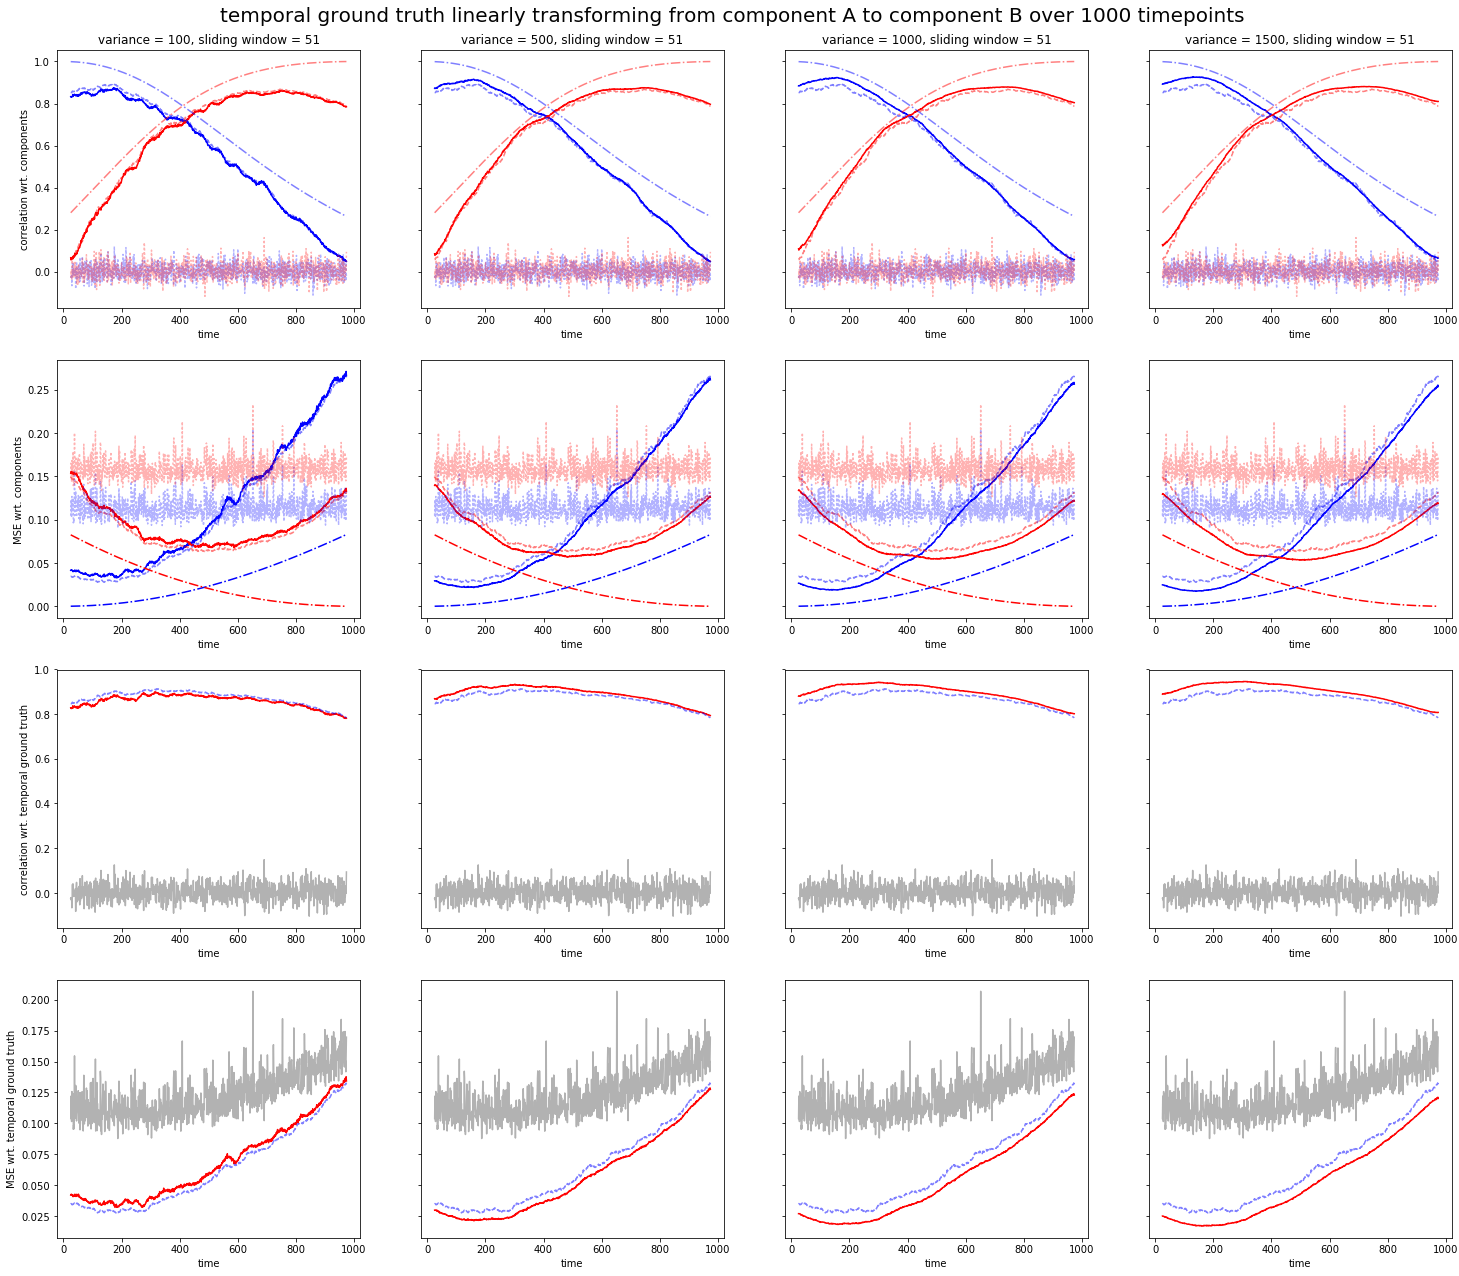
\includegraphics[width=1\textwidth]{../figures/SyntheticTesting/ramp1000t4var.png}
\label{fig:ramp1000t4var}
(a) In the first row, solid lines show the correlation between the two terminal correlations and TimeCorr results; dotted, sliding window results; dot-dashed, ground truth. (b) In the second row, solid lines show mean squared error(MSE) between the two terminal correlations and TimeCorr results; dotted, sliding window results; dot-dashed, ground truth. (c) In the third row, the solid line shows correlation between temporal ground truth and TimeCorr results; dotted, sliding window results; gray, random guess. (d) In the fourth row, the solid line shows MSE between temporal ground truth and TimeCorr results; dotted line, sliding window results; gray, random guess. (e) The columns represent TimeCorr implementations with a different Gaussian variances. (f) In the first two rows, the blue lines represent the relationship between recovered result and the left terminal correlation; red line, right terminal correlation.
\end{figure}

First, 100 ramping datasets with 1000 time points were generated to produce a gradual linear transition between two distinct correlation structures. The average results are displayed in Figure \ref{fig:ramp1000t4var}. At Gaussian variance equal to 100, TimeCorr shows very similar performance with the sliding window method with a window length of 51, albeit TimeCorr results do not come at the expense of extensive data-loss. When the Gaussian variance of TimeCorr is increased beyond 100, the TimeCorr results' advantages over the sliding window result immediately becomes obvious in both MSE and their correlation with the temporal ground truths. This phenomenon is most evident in the third and fourth row, where the TimeCorr results consistently shows higher correlation and lower MSE with the ground truth at almost every time point.

\begin{figure}[!htb]
\caption{Testing on 500 time point ramping dataset}
\includegraphics[width=1\textwidth]{../figures/SyntheticTesting/ramp500t4var.png}
\label{fig:ramp500t4var}
(a) In the first row, solid lines show the correlation between the two terminal correlations and TimeCorr results; dotted, sliding window results; dot-dashed, ground truth. (b) In the second row, solid lines show mean squared error(MSE) between the two terminal correlations and TimeCorr results; dotted, sliding window results; dot-dashed, ground truth. (c) In the third row, the solid line shows correlation between temporal ground truth and TimeCorr results; dotted, sliding window results; gray, random guess. (d) In the fourth row, the solid line shows MSE between temporal ground truth and TimeCorr results; dotted line, sliding window results; gray, random guess. (e) The columns represent TimeCorr implementations with a different Gaussian variances. (f) In the first two rows, the blue lines represent the relationship between recovered result and the left terminal correlation; red line, right terminal correlation.
\end{figure}

TimeCorr's performance advantage is further verified by the testing results from 100 ramping datasets of 500 time points, where the linear transitions between the two distinct terminal correlation structures are accelerated from the 1000 time point datasets. The average results are shown in Figure \ref{fig:ramp500t4var}. In contrast to the results from the 1000 time point datasets, the performance difference is more evident in the results from the 500 time point datasets. As the temporal ground truth correlation linearly transitions from the left terminal correlation structure to the right terminal correlation structure within 500 time points, the rate of change at each time point is much greater than that of the 1000 time point dataset. Under these conditions, the TimeCorr results consistently shows significantly higher correlation and lower MSE with the temporal ground truths than the sliding window results. TimeCorr's superior performance here indicates that it is better at recovering rapidly changing dynamic correlation structures than the sliding window approach. In addition, the results does not seem to change significantly from the 500 variance TimeCorr implementation to the 1500 variance TimeCorr implementation, which might be due to the variance exceeding the dataset time length.

\begin{figure}[!htb]
\caption{Testing on 100 time point ramping dataset}
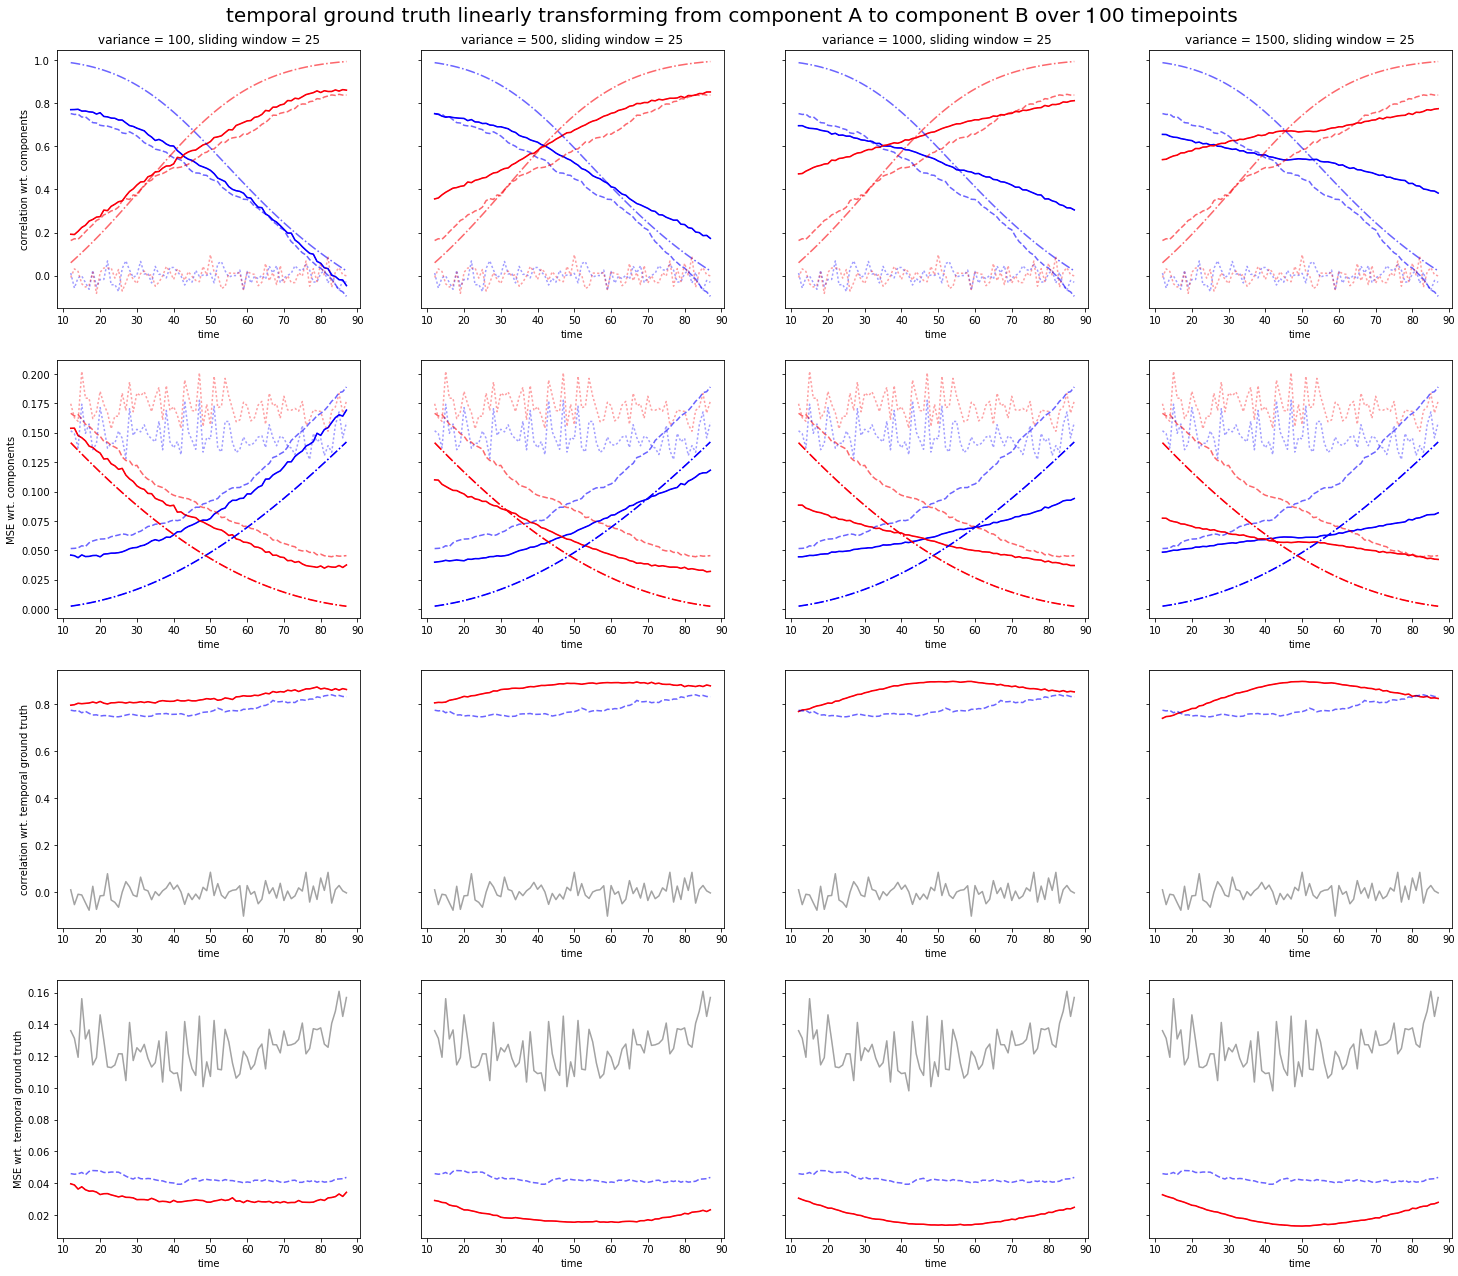
\includegraphics[width=1\textwidth]{../figures/SyntheticTesting/ramp100t4var.png}
\label{fig:ramp100t4var}
(a) In the first row, solid lines show the correlation between the two terminal correlations and TimeCorr results; dotted, sliding window results; dot-dashed, ground truth. (b) In the second row, solid lines show mean squared error(MSE) between the two terminal correlations and TimeCorr results; dotted, sliding window results; dot-dashed, ground truth. (c) In the third row, the solid line shows correlation between temporal ground truth and TimeCorr results; dotted, sliding window results; gray, random guess. (d) In the fourth row, the solid line shows MSE between temporal ground truth and TimeCorr results; dotted line, sliding window results; gray, random guess. (e) The columns represent TimeCorr implementations with a different Gaussian variances. (f) In the first two rows, the blue lines represent the relationship between recovered result and the left terminal correlation; red line, right terminal correlation.
\end{figure}

To further verify the advantages of TimeCorr in recovering highly dynamic correlation structures and the limitations of changing TimeCorr Gaussian variance in datasets with short time lengths, we conducted analysis on 100 ramping datasets of only 100 time points, where the linear transitions between the two distinct terminal correlation structures are further accelerated from the 500 time point datasets. The results are shown in Figure \ref{fig:ramp100t4var} and confirm our observations from the previous tests: the TimeCorr approach consistently out-performs the sliding window approach in every setup and TimeCorr's performance stagnates/worsens as its Gaussian variance increases beyond the total time length of the dataset. These results further consolidates TimeCorr's superiority over the sliding window method in recovering highly dynamic correlation structures. In addition, we gained very useful insight on how to select Gaussian variance for TimeCorr to produce the best recovery results: the most stable results seem to come from a Gaussian variance equal to the lesser between the total time length and 1000 time points.

\begin{figure}[!htb]
\caption{Testing on 1000 time point ramping dataset}
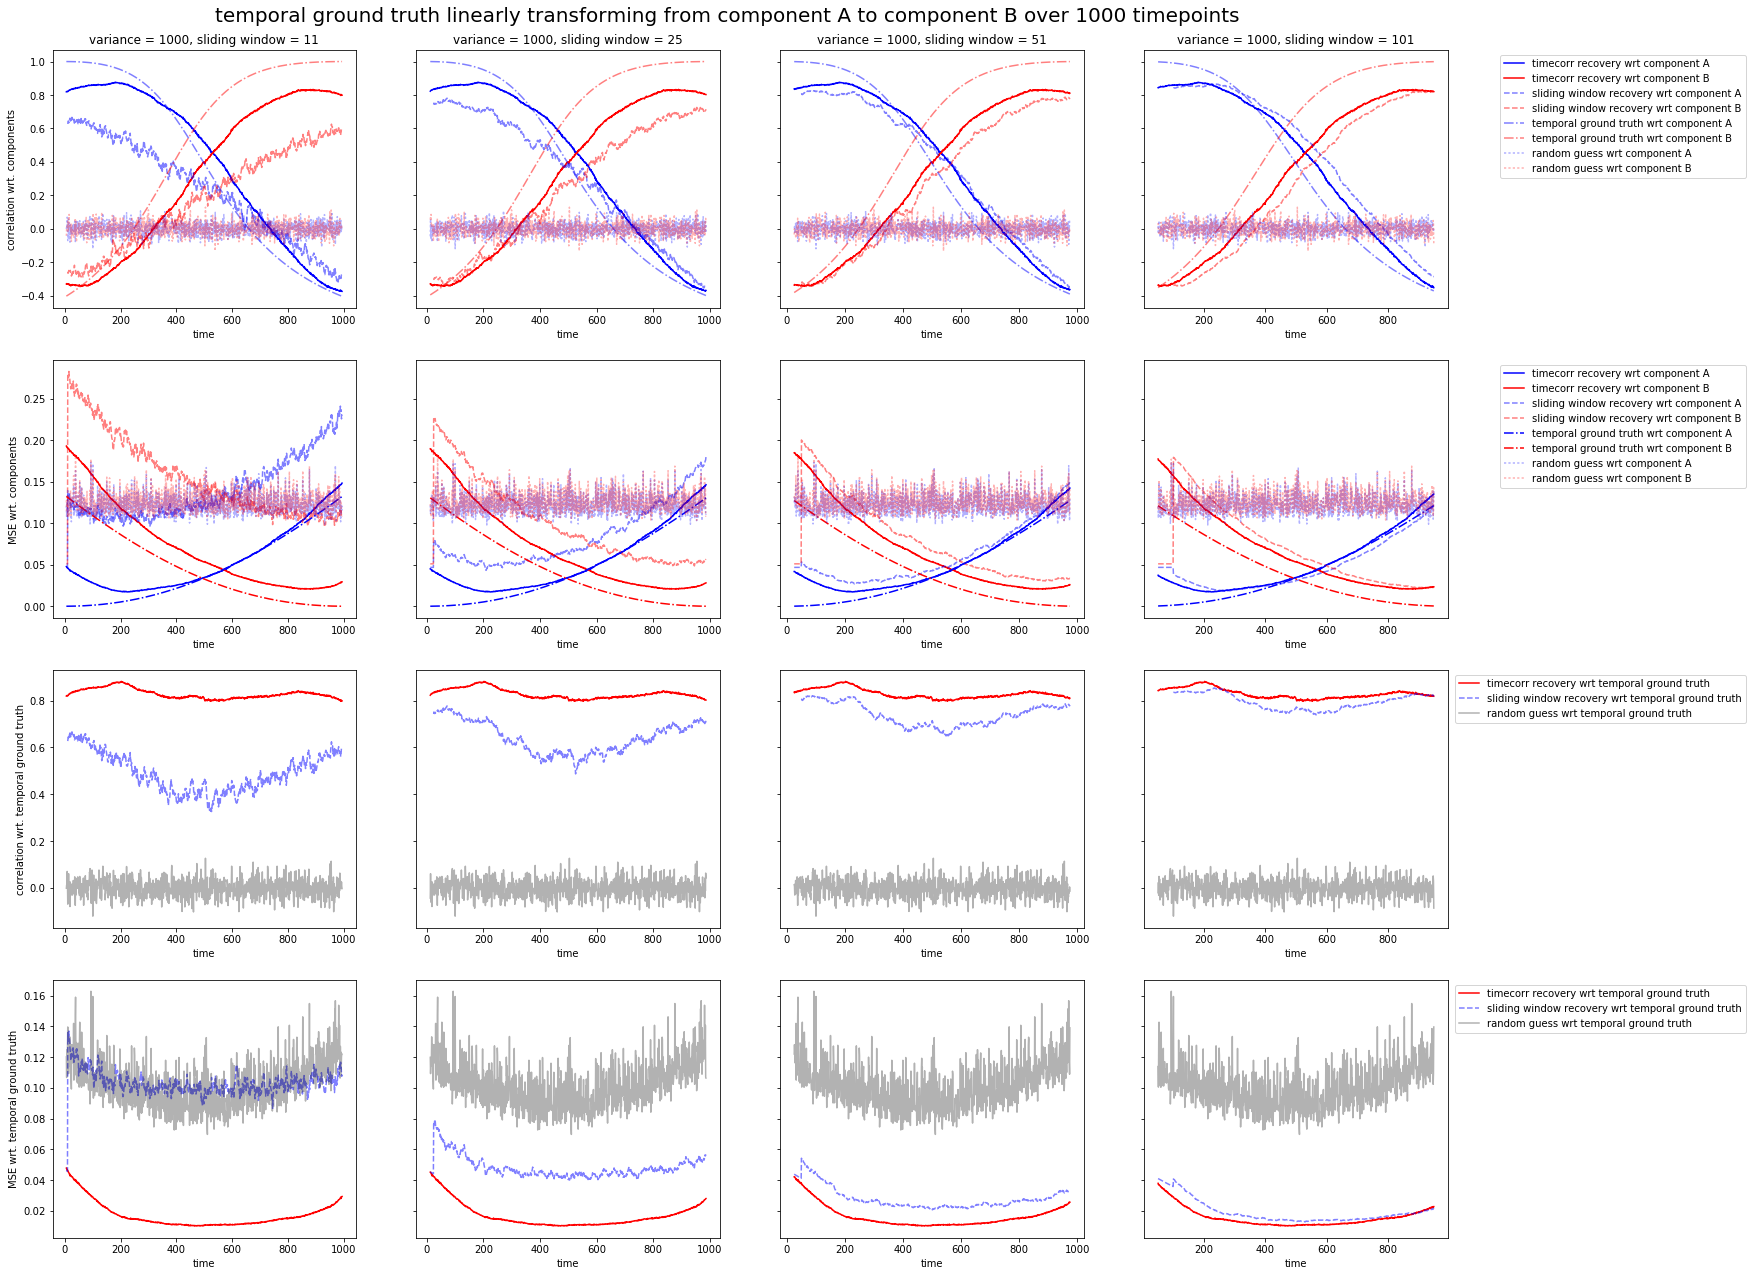
\includegraphics[width=1\textwidth]{../figures/SyntheticTesting/ramp1000t4slide.png}
\label{fig:ramp1000t4slide}
(a) In the first row, solid lines show the correlation between the two terminal correlations and TimeCorr results; dotted, sliding window results; dot-dashed, ground truth. (b) In the second row, solid lines show mean squared error(MSE) between the two terminal correlations and TimeCorr results; dotted, sliding window results; dot-dashed, ground truth. (c) In the third row, the solid line shows correlation between temporal ground truth and TimeCorr results; dotted, sliding window results; gray, random guess. (d) In the fourth row, the solid line shows MSE between temporal ground truth and TimeCorr results; dotted line, sliding window results; gray, random guess. (e) The columns represent different sliding window implementations with varying window lengths. (f) In the first two rows, the blue lines represent the relationship between recovered result and the left terminal correlation; red line, right terminal correlation.
\end{figure}

Lastly, to demonstrate TimeCorr's advantage over the sliding window approach generalizes to all setups, we conducted an analysis on 100 ramping datasets, each containing 1000 time points, to compare TimeCorr with sliding window implementations of varying window length. The results are shown in Figure \ref{fig:ramp1000t4slide}. The TimeCorr setup used for comparison has a Gaussian variance of 1000, a standard setup with average performance among all TimeCorr setups in the previous tests. From the graphs, we can see that the performance of sliding window generally increases as the window length increases, but the rate of improvement decreases dramatically past a window length of 51 time points (marginal improvement when an additional 50 time points is added to the window length). In addition, the performance of the sliding window approach at a window length of 11 time points is underwhelming in comparison with the TimeCorr approach. As the window length increases to 101 time points, the correlation and MSE between the sliding window result and temporal ground truths gradually nears the performance of the standard TimeCorr implementation. However, a window length of 101 time points is equivalent to around $10\%$ of the time length of most fMRI datasets. Losing $10\%$ of the information for calculation of functional connectivity at each level is impractical for explorations of high level brain dynamics. For the above reasons, we chose TimeCorr as the more preferable method of functional connectivity calculation for our High-Order Brain Dynamics Model.


\subsection{Testing Inter-Subject Functional Connectivity using TimeCorr}
Confident with the TimeCorr approach's ability to recover the dynamic correlation structures of single subject datasets, we proceeded to test TimeCorr's performance in recovering inter-subject functional connectivity in multi-subject synthetic datasets. In practical scenarios, fMRI datasets always contain a significant amount of noise from non stimulus-driven neural activities. Therefore, to simulate realistic human brain activities, we added different levels of random noise to the synthetic datasets to gauge the robustness of TimeCorr ISFC in recovering stimulus-related functional connectivity. The noise levels we experimented with were on the order of magnitudes of $10\%$ (0.1), $100\%$(1), $1000\%$(10) and $10000\%$(100) of the average activation magnitude. Running TimeCorr with Gaussian variance of 1000 time points and a sliding window setup with a window length of 25 time point on 100 ramping datasets, each containing 300 time points, we obtained the results displayed in Figure \ref{fig:t300slide25var1000}.

\begin{figure}[!htb]
\caption{Testing on 100 time point ramping dataset}
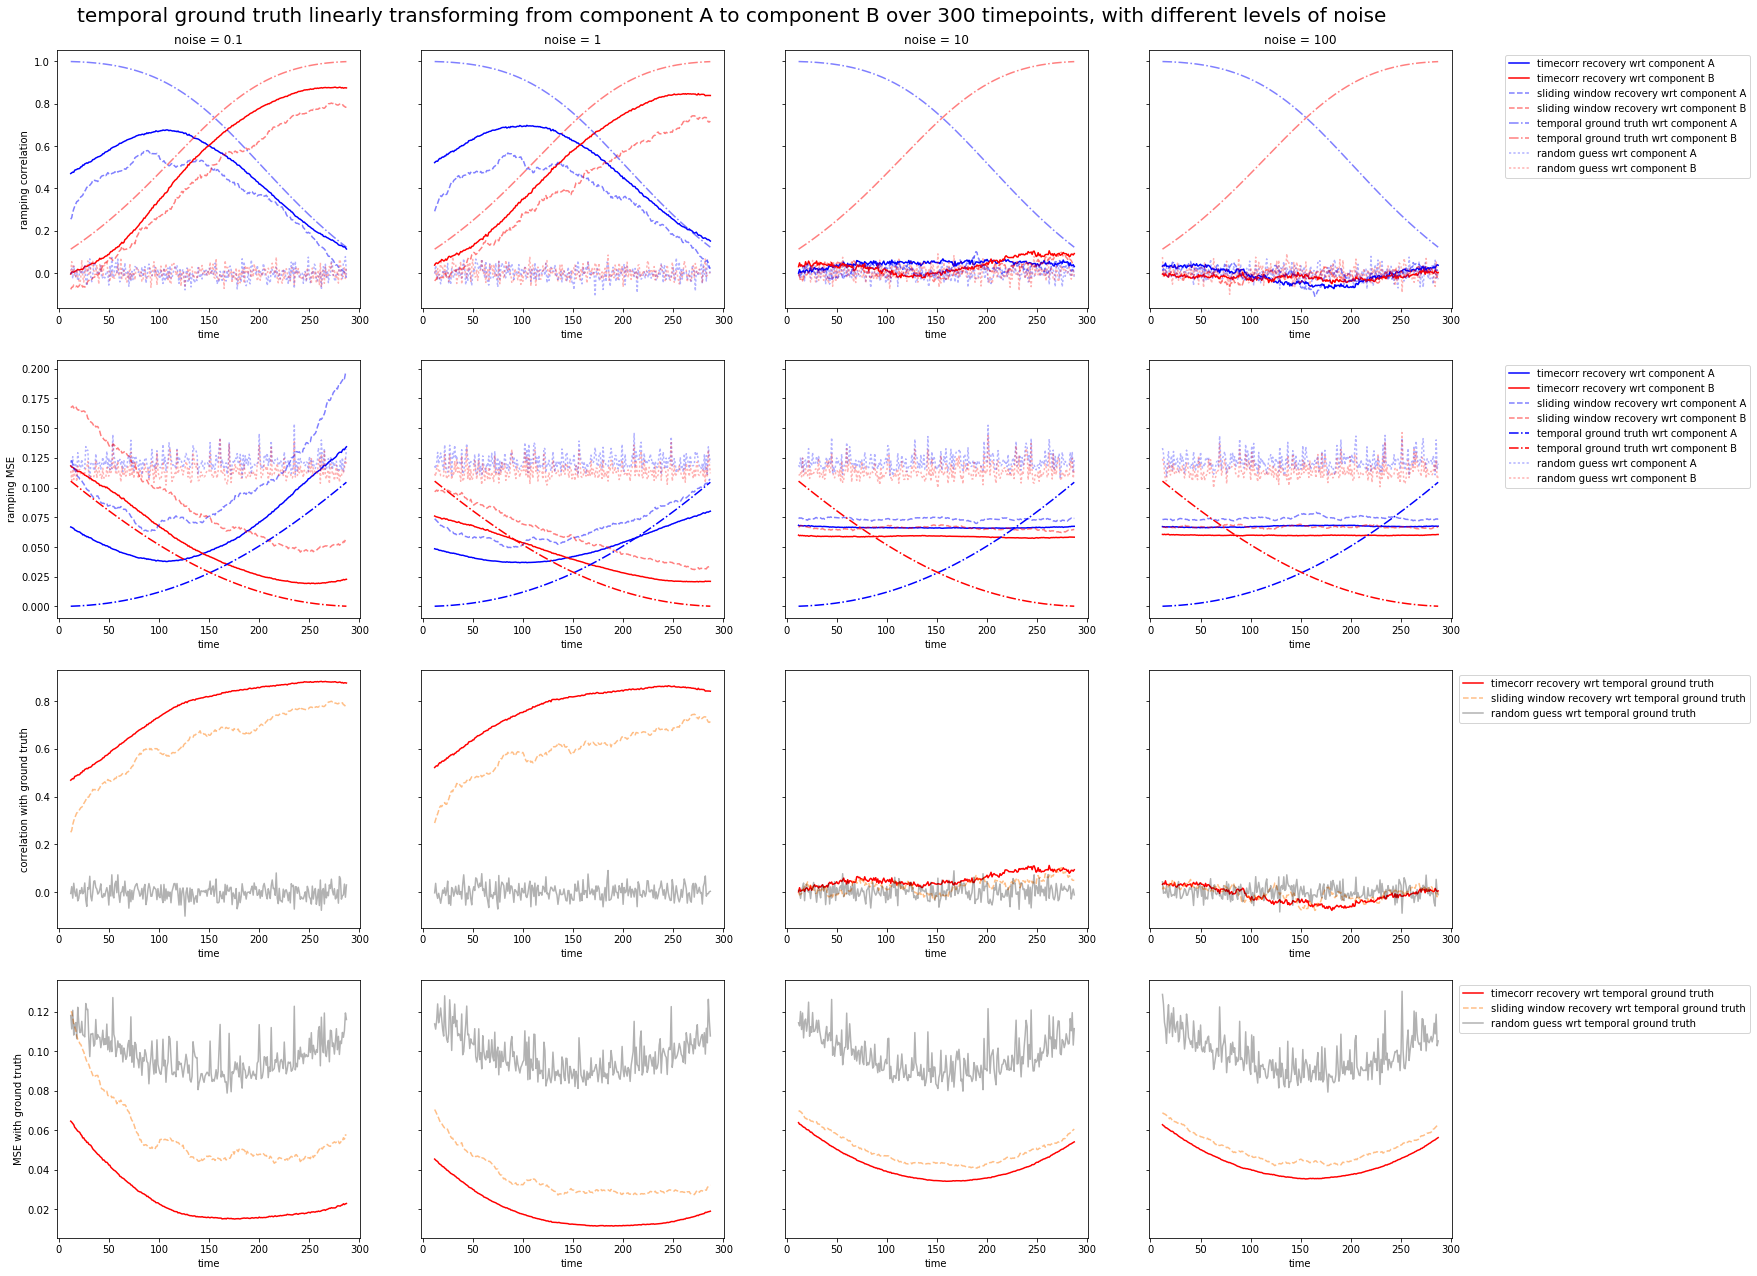
\includegraphics[width=1\textwidth]{../figures/ISFC/t300slide25var1000.png}
\label{fig:t300slide25var1000}
(a) In the first row, solid lines show the correlation between the two terminal correlations and TimeCorr results; dotted, sliding window results; dot-dashed, ground truth. (b) In the second row, solid lines show mean squared error(MSE) between the two terminal correlations and TimeCorr results; dotted, sliding window results; dot-dashed, ground truth. (c) In the third row, the solid line shows correlation between temporal ground truth and TimeCorr results; dotted, sliding window results; gray, random guess. (d) In the fourth row, the solid line shows MSE between temporal ground truth and TimeCorr results; dotted line, sliding window results; gray, random guess. (e) The columns represent recovery results from datasets with varying noise levels. (f) In the first two rows, the blue lines represent the relationship between recovered result and the left terminal correlation; red line, right terminal correlation.
\end{figure}

The results show that TimeCorr is able to retrieve the stimulus-driven dynamic correlation structure with relatively high accuracy at low(0.1) to medium(1) noise levels, but fails to recover any meaningful information when the noise level is too high(10 and 100). These results highlight the difficulty of recovering stimulus-driven correlation structures when the subjects display weak cognitive response to the stimulus. However, when the stimuli is able to evoke reasonably strong cognitive response from the subject, TimeCorr can effectively recover the stimuli-driven dynamic correlation structures with relatively high accuracy.

In addition, due to the limited number of total time points in the dataset, we chose to use a sliding window setup with a window length of 25 time points. When comparing the correlation and MSE between their results and the temporal ground truths, the TimeCorr approach distinctly outperforms the sliding window method in every situation. Furthermore, as the amount of noise increases, the performance of the sliding window approach deteriorates more noticeably than that of the TimeCorr approach. These contrasts further consolidates TimeCorr as the superior choice for functional connectivity calculations.


\subsection{Decoding Analysis using TimeCorr ISFC}
Next, we evaluated how brain dynamics is represented by each level of high-order inter-subject functional connectivity (ISFC). On top of the PCA reduced activations from fMRI datasets, we used the TimeCorr Level Up function to calculate 9 levels of high-order functional connectivity, each containing an equal number of voxels. Next, we conducted decoding analysis on each level of information, from PCA reduced fMRI activations ($0^{th}$ order ISFC) and the ISFC of the PCA reduced activations ($1^{st}$ order ISFC) to the ISFC of the 9th order functional connectivity ($10^{th}$ order ISFC). Three TimeCorr setups were implemented---each with Gaussian variances of 1000 time points, 10 time points, or 1 time point---to comprehensively understand the decoding capability of each level under varying resolutions.

Three different datasets were used for this analysis: Sherlock, Pieman, and Forrest. Detailed descriptions for each dataset are included in each subsection. For each TimeCorr setup for each dataset, we conducted 100 repetitions of decoding analysis with different random group divisions. All of the following results are the average of 100 repetitions.

\subsubsection{Description for the Pieman Dataset}

The stimuli for this experiment were derived from a 7 minute recording of the ``Pie Man" story by Jim O'Grady. The experiment was conducted on native English speakers with normal hearing, and was divided into four testing conditions: 36 subjects listened to the story from beginning to end, and were labelled as the ``intact" group; 18 subjects listened to a version of the story where the paragraphs were scrambled randomly, and were labelled as the ``paragraph" group; 36 subjects listened to a version of the story where the words were scrambled randomly, and were labelled as the ``word" group; lastly, 36 subjects did not listen to anything and stayed in resting state throughout the experiment, and were labelled as the ``resting" group. 12 seconds of neutral music and 3 seconds of silence preceded and 15 seconds of silence followed each playback in all conditions. The data from music and silence periods were discarded from all analyses.\citep{hasson2016}

\subsubsection{Description for the Forrest Dataset}
The stimuli for this experiment is a two-hour presentation of an audio-only version of the Hollywood feature film ``Forrest Gump" made specifically for a visually impaired audience. The movie was divided into eight 15-minute sessions with breaks in-between, and presented to 20 subjects with normal hearing. During each session, brain activities centered on the auditory cortices in both brain hemisphere and the frontal and posterior portions of the brain were recorded into high resolution 7-Tesla fMRI datasets.\citep{Hanke2014}

\subsubsection{Description for the Sherlock Dataset}
Sixteen participants (17 were described in the original paper, but 1 was removed for this dataset due to a small amount of missing data at the end of the movie scan.) were presented with a 50-minute segment of the audio-visual movie Sherlock (BBC) while undergoing fMRI scan. Before each viewing, the subjects were informed that they would later need to describe the contents of movie. Following the viewing, participants were asked to describe aloud what they recalled of the movie in as much detail as they could while undergoing brain imaging, with no visual input or experimenter guidance. Participants were allowed to speak on any aspect of the movie for as long as they wished, while their speech was recorded with an fMRI-compatible microphone. \citep{Chen2017}

\subsubsection{Results}
\begin{enumerate}
\item The average results for each TimeCorr setup implemented on the Pieman dataset are displayed in Figure \ref{fig:piemanDC1000}, \ref{fig:piemanDC10}, and \ref{fig:piemanDC1}.
\item The average results for each TimeCorr setup implemented on the Forrest dataset are displayed in Figure \ref{fig:forrestDC1000}, Figure \ref{fig:forrestDC10} and Figure \ref{fig:forrestDC1}.
\item The average results for each TimeCorr setup implemented on the Sherlock dataset are displayed in Figure \ref{fig:sherlockDC1000}, Figure \ref{fig:sherlockDC10} and Figure \ref{fig:sherlockDC1}.
\end{enumerate}

\begin{figure}[!htb]
\caption{Decoding Analysis using TimeCorr with variance of 1000 time points (Pieman)}
\centering
\includegraphics[width=0.6\textwidth]{../figures/Intra-Level-Decoding-Analysis/1000V/pieman.png}
\label{fig:piemanDC1000}
\end{figure}

\begin{figure}[!htb]
\caption{Decoding Analysis using TimeCorr with variance of 10 time points (Pieman)}
\centering
\includegraphics[width=0.6\textwidth]{../figures/Intra-Level-Decoding-Analysis/10V/pieman.png}
\label{fig:piemanDC10}
\end{figure}

\begin{figure}[!htb]
\caption{Decoding Analysis using TimeCorr with variance of 1 time point (Pieman)}
\centering
\includegraphics[width=0.6\textwidth]{../figures/Intra-Level-Decoding-Analysis/1V/pieman.png}
\label{fig:piemanDC1}
\end{figure}

\begin{figure}[!htb]
\caption{Decoding Analysis using TimeCorr with variance of 1000 time points (Forrest)}
\centering
\includegraphics[width=0.6\textwidth]{../figures/Intra-Level-Decoding-Analysis/1000V/forrest.png}
\label{fig:forrestDC1000}
\end{figure}

\begin{figure}[!htb]
\caption{Decoding Analysis using TimeCorr with variance of 10 time points (Forrest)}
\centering
\includegraphics[width=0.6\textwidth]{../figures/Intra-Level-Decoding-Analysis/10V/forrest.png}
\label{fig:forrestDC10}
\end{figure}

\begin{figure}[!htb]
\caption{Decoding Analysis using TimeCorr with variance of 1 time point (Forrest)}
\centering
\includegraphics[width=0.6\textwidth]{../figures/Intra-Level-Decoding-Analysis/1V/forrest.png}
\label{fig:forrestDC1}
\end{figure}

\begin{figure}[!htb]
\caption{Decoding Analysis using TimeCorr with variance of 1000 time points (Sherlock)}
\centering
\includegraphics[width=0.6\textwidth]{../figures/Intra-Level-Decoding-Analysis/1000V/sherlock.png}
\label{fig:sherlockDC1000}
\end{figure}

\begin{figure}[!htb]
\caption{Decoding Analysis using TimeCorr with variance of 10 time points (Sherlock)}
\centering
\includegraphics[width=0.6\textwidth]{../figures/Intra-Level-Decoding-Analysis/10V/sherlock.png}
\label{fig:sherlockDC10}
\end{figure}

\begin{figure}[!htb]
\caption{Decoding Analysis using TimeCorr with variance of 1 time point (Sherlock)}
\centering
\includegraphics[width=0.6\textwidth]{../figures/Intra-Level-Decoding-Analysis/1V/sherlock.png}
\label{fig:sherlockDC1}
\end{figure}

When comparing our results with previous efforts, we can see that the decoding accuracy we achieved on the first order ISFC for the Pieman dataset using TimeCorr-based methods is significantly higher across all TimeCorr setups \citep{jeremy2017}. As higher decoding accuracy is a strong indication of the richness of stimulus-driven activities within a dataset, our improved results further confirm that TimeCorr-based methods are superior in the recovery of stimulus-driven correlation structure in fMRI datasets. Furthermore, the decoding accuracy we achieved on PCA reduced fMRI data is significantly higher than the decoding accuracy obtained from HTFA reduced datasets, indicating that PCA is more effective in preserving dynamic structure than HTFA and justifying it's usage in our level up method.

Another important observation that is consistent across results from all three datasets is that the higher order ISFCs actually produced lower decoding accuracy. This result was unexpected as brain dynamics across subjects should intuitively become more similar at higher orders. One possible explanation for this is, although the high order ISFC still contain information about stimulus-driven brain activities, there seems to have been a small amount of information loss in each level up process, leading to slightly lower classification accuracy. However, although higher order ISFCs display weaker decoding capabilities than ISFCs at lower level, our hypothesis is that each order of ISFC contains distinct information about brain dynamics. If this is the case, then a mixture of all orders of ISFC will potentially have stronger decoding performance than that of ISFC at any single level.

We also suspected that TimeCorr temporal resolution had some influence on the results, which is why our analysis of each dataset consists of a variety of different TimeCorr setups. We hypothesize that if the Gaussian averaging process in TimeCorr caused information loss at each ``level up", the loss would intuitively grow exponentially as we reach higher orders of functional connectivity. Therefore, TimeCorr with Gaussian variances of 1000 time points, 10 time points and 1 time point were chosen to explore if variation in TimeCorr temporal resolution would affect the distribution of decoding accuracy across different levels. However, looking at the results across all three datasets, we do not notice a significant decrease in the rate of decoding accuracy deterioration when the TimeCorr resolution shifts from a variance of 1000 time points to a variance of 1 time point. On the contrary, there does not seem to be a linear relationship between the decoding accuracy at higher levels and the temporal resolution of TimeCorr: e.g. the decoding accuracy of first order ISFC in the Pieman dataset increased when TimeCorr variance decreased from 1000 time points to 10 time points, but decreased when the TimeCorr variance decreased further to 1 time point (a phenomenon also observed in the Forrest results). These observations indicate that the Guassian averaging process in TimeCorr is not the main culprit of information loss.

The results from the Pieman dataset showed that the decoding accuracy of lower orders of ISFC increasing drastically when the TimeCorr temporal resolution increased from a Gaussian variance of 1000 time points to a Gaussian variance of 10 time points, but undergoing a decrease as the temporal resolution was increased further to a Gaussian variance of 1 time point. The results from Sherlock and Forrest datasets also show similar patterns. Additionally, we observe that, as the TimeCorr temporal resolution increases from Gaussian variance of 1000 time points to Gaussian variance of 1 time point, the decoding accuracy of higher order ISFCs of the Pieman dataset seem to show a marginal increase, a pattern not replicated by the results from the Forrest dataset.

We reason that the variation in decoding capabilities across different TimeCorr temporal resolutions may be attributed to different levels of focus revealing different information about the dynamics. As revealed in single subject TimeCorr testing, when the resolution is high (low Gaussian variance), the recovered correlation structures tend to have higher temporal accuracy, whereas low resolution TimeCorr (high Gaussian variance) can recover dynamic correlations with more stability. Therefore, when high resolution TimeCorr is used to decode the datasets, the ISFC-based brain information (high order brain connectivities) will contain more accurate information on the temporal correlation structure, thereby increasing time-point-to-time-point decoding accuracy. However, when the temporal resolution of TimeCorr is too high (Gaussian variance of 1 time point), TimeCorr will tunnel-vision on a very narrow neighborhood of time points for its functional connectivity calculations, and thus fail to incorporate enough information to recover any meaningful dynamic correlation patterns.

Lastly, when comparing between results under different stimulus conditions (intact, paragraph, word, resting) within the Pieman dataset, we can see that as the complexity and integrity of the stimulus decreases, the decoding accuracy decreases for all orders of functional connectivity. This makes sense as the human brain should intuitively produce more potent cognitive response to more coherent and meaningful stimuli (intact), weaker response to scrambled and irrational stimuli (paragraph, word), and little to no response to no stimuli (resting). One anomaly exists in the results from the TimeCorr implementation with a Gaussian variance of 1 time point, where the decoding accuracy of the first order ISFC in the paragraph condition exceeded that of the intact condition. However, this behavior becomes understandable after taking into consideration the results from the TimeCorr implementation with a Gaussian variance of 10 time points: while the decoding accuracy for the first order ISFC of the paragraph condition only showed marginal decrease, the decoding accuracy of the first order ISFC of the intact condition decreased drastically when the TimeCorr Gaussian variance changed from 10 time points to 1 time point. As discussed previously, when the TimeCorr's temporal resolution is too high, it may fail to include enough global information to recovery meaningful dynmaic correlation structures. As the functional connectivity under the intact condition possesses more structure and coherency, it may be suffer greater deterioration than the functional connectivity from the paragraph condition when subjected to over-high temporal resolution, thus explaining the anomaly.


\subsection{Multi-Level Mixture Analysis}
To verify our hypothesis that the functional connectivity at each level represent non-overlapping sources of stimulus-relevant cognitive information that could potentially complement each other, we designed the Multi-Level Mixture Analysis. This analysis constructs a mixture model incorporating information from multiple orders of ISFC, and compares its decoding capabilities with that of ISFC at each individual level.

Given a fMRI dataset for $S$ subjects, each possessing $T$ time points and $V$ voxels, to construct the Multi-Level Mixture Model:
\begin{enumerate}
\item Choose the desired number of levels of functional connectivities $L$ and the appropriate Gaussian variance for TimeCorr.
\item Use the TimeCorr Level Up method to obtain all level functional connectivites for each subject.
\item Randomly divide the subjects in to four equal groups $A_1$, $A_2$, $B_1$ and $B_2$.
\item For each group, use the Multi-Subject TimeCorr ISFC method to compute the inter-subject functional connectivity for each level
\item Compute correlation matrices for each level for A and B (i.e. for group A, correlate A1's features at each time point with A2's features at each time point; similarly for group B). This yields one correlation matrix for group A and another for group B, for each level (including level 0). So if $L=10$, this process would yield 11 correlation matrices for A and another 11 for B.
\item Apply Fisher Z-transform (r2z) on all of the correlation matrices. The transformed correlation matrices are labelled $z_{A0}, z_{A1}, z_{A2}, ..., z_{B0}, z_{B1}, z_{B2}, ..., z_{B10}$, where $z_{A0}$ represent the Fisher Z-transformed correlation matrix for level 0 of group A.
\item Use constrained optimization by linear approximation (COBYLA) on the correlation matrices of group A to compute the optimal weight matrix w to be used for decoding, where $w$ will be applied to the Fisher Z-transformed matrices in the manner of the following equation:
\begin{align*}
\text{decoding\_matrix\_A} = z2r(w[0]*z_A0 + w[1]*z_A1 + w[2]*z_A2 + ... + w[10]*z_A10)
\end{align*}
where $z2r$ is the Inverse Fisher Z-transformation to convert the weighted sum into the its proper correlation form. Intuitively, this step seeks to find the w that maximizes the decoding accuracy using decoding\_matrix\_A.
\item Use the same z2r(weighted z-transformed sum) formula and the optimal weights from the previous step to compute decoding accuracy for group B
\item Output w and group B's decoding accuracy
\end{enumerate}

Three TimeCorr setups were implemented---each with Gaussian variances of 1000 time points, 10 time points, or 1 time point---to comprehensively understand the decoding capability of the mixture model and each individual level under varying resolutions. In addition, similar to the single level decoding analysis conducted previously, three different datasets were used for this analysis: Sherlock, Pieman, and Forrest. For each TimeCorr setup for each dataset, we conducted 100 repetitions of decoding analysis with different random group divisions. All of the following results are the average of 100 repetitions.

Results:
\begin{enumerate}
\item The average results for each TimeCorr setup implemented on the Pieman dataset are displayed in Figure \ref{fig:piemanMM1000}, \ref{fig:piemanMM10}, and \ref{fig:piemanMM1}.
\item The average results for each TimeCorr setup implemented on the Forrest dataset are displayed in Figure \ref{fig:forrestMM1000}, Figure \ref{fig:forrestMM10} and Figure \ref{fig:forrestMM1}.
\item The average results for each TimeCorr setup implemented on the Sherlock dataset are displayed in Figure \ref{fig:sherlockMM1000}, Figure \ref{fig:sherlockMM10} and Figure \ref{fig:sherlockMM1}.
\end{enumerate}

\begin{figure}[!htb]
\caption{Multi-Level Mixture Analysis using TimeCorr with variance of 1000 time points}
\centering
\includegraphics[width=1\textwidth]{../figures/Multi-Level-Mixture-Analysis/1000V/pieman-weights.png}
\includegraphics[width=1\textwidth]{../figures/Multi-Level-Mixture-Analysis/1000V/pieman-accuracy.png}
\label{fig:piemanMM1000}
\end{figure}

\begin{figure}[!htb]
\caption{Multi-Level Mixture Analysis using TimeCorr with variance of 10 time points}
\centering
\includegraphics[width=1\textwidth]{../figures/Multi-Level-Mixture-Analysis/10V/pieman-weights.png}
\includegraphics[width=1\textwidth]{../figures/Multi-Level-Mixture-Analysis/10V/pieman-accuracy.png}
\label{fig:piemanMM10}
\end{figure}

\begin{figure}[!htb]
\caption{Multi-Level Mixture Analysis using TimeCorr with variance of 1 time point}
\centering
\includegraphics[width=1\textwidth]{../figures/Multi-Level-Mixture-Analysis/1V/pieman-weights.png}
\includegraphics[width=1\textwidth]{../figures/Multi-Level-Mixture-Analysis/1V/pieman-accuracy.png}
\label{fig:piemanMM1}
\end{figure}

\begin{figure}[!htb]
\caption{Multi-Level Mixture Analysis using TimeCorr with variance of 1000 time points}
\centering
\includegraphics[width=1\textwidth]{../figures/Multi-Level-Mixture-Analysis/1000V/forrest.png}
\label{fig:forrestMM1000}
\end{figure}

\begin{figure}[!htb]
\caption{Multi-Level Mixture Analysis using TimeCorr with variance of 10 time points}
\centering
\includegraphics[width=1\textwidth]{../figures/Multi-Level-Mixture-Analysis/10V/forrest.png}
\label{fig:forrestMM10}
\end{figure}

\begin{figure}[!htb]
\caption{Multi-Level Mixture Analysis using TimeCorr with variance of 1 time point}
\centering
\includegraphics[width=1\textwidth]{../figures/Multi-Level-Mixture-Analysis/1V/forrest.png}
\label{fig:forrestMM1}
\end{figure}

\begin{figure}[!htb]
\caption{Multi-Level Mixture Analysis using TimeCorr with variance of 1000 time points}
\centering
\includegraphics[width=1\textwidth]{../figures/Multi-Level-Mixture-Analysis/1000V/sherlock.png}
\label{fig:sherlockMM1000}
\end{figure}

\begin{figure}[!htb]
\caption{Multi-Level Mixture Analysis using TimeCorr with variance of 10 time points}
\centering
\includegraphics[width=1\textwidth]{../figures/Multi-Level-Mixture-Analysis/10V/sherlock.png}
\label{fig:sherlockMM10}
\end{figure}

\begin{figure}[!htb]
\caption{Multi-Level Mixture Analysis using TimeCorr with variance of 1 time point}
\centering
\includegraphics[width=1\textwidth]{../figures/Multi-Level-Mixture-Analysis/1V/sherlock.png}
\label{fig:sherlockMM1}
\end{figure}

With each implementation of the Multi-Level Mixture Model, the subjects are divided into two equal groups, one for training and one for testing. As a result, we observe that training and testing using only half of the subjects caused the decoding accuracy to be a lot lower than when using the entire dataset. From a mathematical perspective, averaging over more subjects brings more stability to the dataset by smoothing out random noises in the dataset and adding emphasis to activities common to all subjects, which are typically stimulus-driven. Therefore, when less subjects are used in the calculation of inter-subject functional connectivity (ISFC), the de-noising effect of averaging is weakened and less emphasis is put on activities that are stimulus-driven, thus causing lower decoding accuracy.

One of the most important observations from the results of Multi-Level Mixture Analysis across all three datasets is that the Mixture Model produces significantly higher decoding accuracy than any single level of ISFC. When taking into consideration our hypothesis from the decoding analysis in the previous section, this is a very direct and compelling proof that different orders of ISFC contain non-overlapping information about brain dynamics and, although individual levels did not produce high classification accuracy, when used in unison can greatly enrich data complexity and increase decoding capabilities.

The importance of each level is further confirmed by optimal weight distribution across all three datasets. While the first order ISFC always has the highest weight, the weight distribution between PCA reduced fMRI activation and higher order connectivities is almost uniform, indicating their equal contribution to the enrichment of stimulus-related information and the improvement in the decoding capability of the dataset. Additionally, we noticed that the optimal weight of the first order ISFC was significantly higher than the rest of the levels, suggesting that a greater amount of stimulus-driven brain dynamics information is contained in this level. The significance of the first order ISFC in the mixture model is also consistent with high resolution results in single level decoding analysis, where first level ISFC achieved the highest decoding accuracy among all levels.

Like in the decoding analysis, we were curious if varying Gaussian variance (changing temporal resolution loss across levels) would influencing the results, therefore we repeated the Multi-Level Mixture Analysis on each dataset with multiple TimeCorr setups. However, the optimal weight distribution qualitatively remained the same in every implementation: the first level ISFC always possesses the highest weight, while other levels always possesses similar weight. This further confirms that, although PCA reduced fMRI activations may sometimes produce higher decoding accuracy at low resolutions, first order ISFC actually contains the most information on brain dynamics that are stimulus-related.

\subsection{High-Order Brain Dynamics Toolbox Benchmark Results}
We wanted to make TimeCorr available to the public as a more effective alternative to the sliding window approach for functional connectivity related research, so we developed a Python toolbox that is available for public download through pip. Detailed documentation on how to use to toolbox is available online at (insert web address after completing documentation).

To make the TimeCorr-derived methods into a practical toolbox that can be widely used by not only specialize laboratories but also the general public, we explored with different optimization and scaling methods to make it less resource intensive. At first, we explored with Cython, an optimizing static compiler that converts Python programs into C for faster implementation. However, we later discovered that multiprocessing has exponentially faster runtimes and scales better with large datasets. We also experimented with a combination of using Cython for preprocessing and multiprocessing for large scale calculation. However, on top of the low runtime achieved using multiprocessing, the time loss from C-Python transitions overshadowed the minimal speed gain from Cython. In the end, we decided to abandon Cython, and rely on multiprocessing as our main means of optimization. In addition, as starting every new process introduces time-loss, we decided that creating a process for each subject instead of for each voxel or time point would result in faster runtime.

\begin{figure}[!htb]
\centering
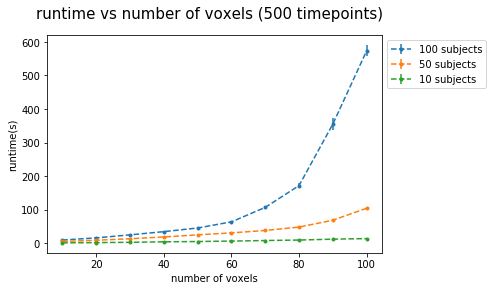
\includegraphics[width=1\textwidth]{../figures/Benchmark/500timepoints.png}
Tests were performed on 2.6 GHz Intel Core i5 processor with 8GB 1600 MHz DDR3 Memory
\label{fig:benchmark}
\end{figure}

The benchmark results of using TimeCorr to calculate inter-subject functional connectivity are shown in Figure \ref{fig:benchmark}. From the graph, we can see that runtime grows exponentially with the number of voxels, but linearly with the number of subjects.

\clearpage
\newpage
\section{Conclusion}
We proposed the High-Order Brain Dynamics Model, a new way to understand brain dynamics by incorporating information in high order inter-subject functional connectivity. In the process, we proposed the TimeCorr method, a lossless alternative to the widely popular sliding window approach for functional connectivity calculation, and the Level Up method, a new means of calculating high order functional connectivity. Through testing on synthetic data, we demonstrated the superiority of the TimeCorr approach over the sliding window approach in recovering temporal functional connectivity. With TimeCorr and Level Up, we had the means to peer into the secrets of the brain through the lens of the High-Order Brain Dynamics Model. First, we calculated 10 orders of functional connectivity from the fMRI data of 3 past studies (Pieman, Forrest and Sherlock). Then, we carried out decoding analysis individually for each order of functional connectivity to understand how well stimulus-driven brain dynamics information is represented at each level. Afterwards, we conducted the Multi-Level Mixture Analysis to understand how information at each order of functional connectivity complements each other. Lastly, we presented all TimeCorr-derived methods as a public toolbox, and demonstrated it's benchmark performance.

Through the lens of the High-Order Brain Dynamics Model, we were able analyze the patterns in higher orders of functional connectivity and achieve a better understanding of stimulus-driven brain dynamics in existing datasets (Pieman, Forrest and Sherlock). In addition, through the construction of the Multi-Level Mixture Model, we were able to find effective ways to optimally combine stimulus-relevant information from multiple orders of functional connectivity into one functional connectivity matrix. This process enriches the amount of stimulus-relevant information in the dataset without creating redundancies, which greatly increases the decoding capabilities of the dataset and has practical applications in many areas:

\begin{enumerate}
\item With more information on how the general population reacts to certain stimuli, we can use the HOBD model to detect cognitive anomalies in patients and potentially detect psychological or mental disorders with more accuracy
\item With more in-depth understanding of how normal people react in certain situations, we can potentially identify criminals through their cognitive response to crime scene reenactments
\item With more stimulus-relevant information from higher order brain dynamics, we increase the ability of  Machine Learning methods to recreate the stimulus (visual, audio, etc), which could potentially give us more knowledge on human perception
\end{enumerate}

Although we were able to increase the amount of stimulus-driven brain dynamics information retrievable from fMRI datasets through the use of the TimeCorr and the Level Up methods, we believe the abrupt decrease in decoding accuracy after the first order ISFC does not accurately represent the amount of information contained in these levels and is indicative of information loss. As our tests proved that TimeCorr is not the main cause for the decrease in decoding accuracy, we hypothesize that the information loss may have partially been caused by PCA dimensionality reduction in the Level Up processes.

To address this issue and to further improve the High-Order Brain Dynamics Model in the future, we intend to experiment with the following options:

\begin{enumerate}
\item Explore alternative dimensionality reduction algorithm, e.g. ICA, t-SNE, MDS, Autoencoders with neural network, etc
\item Explore alternative ways of calculating functional connectivity, e.g. Gaussian Process
\item Explore alternative ways of representing high order functional connectivity, e.g. Neural Networks
\item Decrease the variance parameter of TimeCorr with each subsequent level, so that the smoothing effect of TimeCorr decreases as the level increases
\item Have the number of voxels after each level up increase with each level, but at a practical rate so that the approach is still scalable to many levels. For example, the number of factors could grow linearly with respect to the level, rather than exponentially (as would happen if we didn't use any dimensionality reduction) or having the number of factors remain constant (as in our current approach).
\end{enumerate}

In conclusion, the HOBD model has provided an accurate and efficient means of examining stimulus-driven brain dynamics at high orders of functional connectivity. We believe the benefits of understanding high order brain connectivity is endless, and we are excitepd to explore new approaches to further improve the HOBD model and further expand the horizon of human brain decoding.

\newpage
\bibliographystyle{apalike}
\bibliography{HOBD}
\end{document}
